%TODO:建立目录、版本控制、可视化训练数据、模型的稳定性!!!!  神经网络??将逾期数看成一个属性


\documentclass[UTF8,a4paper,10pt]{ctexart}
\usepackage[left=2.50cm, right=2.50cm, top=2.50cm, bottom=2.50cm]{geometry} %页边距

\CTEXsetup[format={\Large\bfseries}]{section} %设置章标题居左
 
 
%%%%%%%%%%%%%%%%%%%%%%%
% -- text font --
% compile using Xelatex
%%%%%%%%%%%%%%%%%%%%%%%
% -- 中文字体 --
%\setmainfont{Microsoft YaHei}  % 微软雅黑
%\setmainfont{YouYuan}  % 幼圆    
%\setmainfont{NSimSun}  % 新宋体
%\setmainfont{KaiTi}    % 楷体
%\setmainfont{SimSun}   % 宋体
%\setmainfont{SimHei}   % 黑体
% -- 英文字体 --
%\usepackage{times}
%\usepackage{mathpazo}
%\usepackage{fourier}
%\usepackage{charter}
\usepackage{helvet}
\usepackage{color}
\usepackage{pdfpages}
 
\usepackage{amsmath, amsfonts, amssymb} % math equations, symbols
\usepackage[english]{babel}
\usepackage{graphicx}   % import figures
\usepackage{url}        % hyperlinks
\usepackage{bm}
\usepackage{caption}         % bold type for equations
\usepackage{multirow}
\usepackage{booktabs}
\usepackage{epstopdf}
\usepackage{epsfig}
\usepackage{algorithm}
\usepackage{algorithmic}
\usepackage{listings}
\renewcommand{\algorithmicrequire}{ \textbf{Input:}}     % use Input in the format of Algorithm  
\renewcommand{\algorithmicensure}{ \textbf{Initialize:}} % use Initialize in the format of Algorithm  
\renewcommand{\algorithmicreturn}{ \textbf{Output:}}     % use Output in the format of Algorithm  
 % Please add the following required packages to your document preamble:
%\usepackage{graphicx}
\usepackage{lscape}
 
\usepackage{fancyhdr} %设置页眉、页脚
%\pagestyle{fancy}
\lhead{}
\chead{}
%\rhead{\includegraphics[width=1.2cm]{fig/ZJU_BLUE.eps}}
\lfoot{}
\cfoot{}
\rfoot{}
 

\usepackage{listings}
\usepackage{color}

\definecolor{dkgreen}{rgb}{0,0.6,0}
\definecolor{gray}{rgb}{0.5,0.5,0.5}
\definecolor{mauve}{rgb}{0.58,0,0.82}

\lstset{ %
  language=Octave,                % the language of the code
  basicstyle=\footnotesize,           % the size of the fonts that are used for the code
  numbers=left,                   % where to put the line-numbers
  numberstyle=\tiny\color{gray},  % the style that is used for the line-numbers
  stepnumber=2,                   % the step between two line-numbers. If it's 1, each line 
                                  % will be numbered
  numbersep=5pt,                  % how far the line-numbers are from the code
  backgroundcolor=\color{white},      % choose the background color. You must add \usepackage{color}
  showspaces=false,               % show spaces adding particular underscores
  showstringspaces=false,         % underline spaces within strings
  showtabs=false,                 % show tabs within strings adding particular underscores
  frame=single,                   % adds a frame around the code
  rulecolor=\color{black},        % if not set, the frame-color may be changed on line-breaks within not-black text (e.g. commens (green here))
  tabsize=2,                      % sets default tabsize to 2 spaces
  captionpos=b,                   % sets the caption-position to bottom
  breaklines=true,                % sets automatic line breaking
  breakatwhitespace=false,        % sets if automatic breaks should only happen at whitespace
  title=\lstname,                   % show the filename of files included with \lstinputlisting;
                                  % also try caption instead of title
  keywordstyle=\color{blue},          % keyword style
  commentstyle=\color{dkgreen},       % comment style
  stringstyle=\color{mauve},         % string literal style
  escapeinside={\%*}{*)},            % if you want to add LaTeX within your code
  morekeywords={*,...}               % if you want to add more keywords to the set
}
%%%%%%%%%%%%%%%%%%%%%%%
%  设置水印
%%%%%%%%%%%%%%%%%%%%%%%
%\usepackage{draftwatermark}         % 所有页加水印
%\usepackage[firstpage]{draftwatermark} % 只有第一页加水印
% \SetWatermarkText{Water-Mark}           % 设置水印内容
% \SetWatermarkText{\includegraphics{fig/ZJDX-WaterMark.eps}}         % 设置水印logo
% \SetWatermarkLightness{0.9}             % 设置水印透明度 0-1
% \SetWatermarkScale{1}                   % 设置水印大小 0-1    
 
\usepackage{hyperref} %bookmarks
\hypersetup{colorlinks, bookmarks, unicode} %unicode
 
 
 
\title{\textbf{信用卡评分建模分析报告}}
\author{ 刘华秋 ,顾逸鸥 ,罗文  }
\date{\today}
 
\begin{document}
\maketitle




\section{问题定义}
\subsection{已知}
1、15000条拥有如下属性的用户数据\newline

% Please add the following required packages to your document preamble:
% \usepackage{graphicx}
% \usepackage[table,xcdraw]{xcolor}
% If you use beamer only pass "xcolor=table" option, i.e. \documentclass[xcolor=table]{beamer}





\begin{table}[htbp]
	\resizebox{\textwidth}{!}{%
		\begin{tabular}{|r|c|l|}
			\hline
			属性名                               & 描述                                                   & 数据类型     \\ \hline
			SeriousDlqin2yrs (label)             & 是否违约(两年内出现逾期超过90天的情况)               & \textbf{Y/N} \\ \hline
			RevolvingUtilizationOfUnsecuredLines & 信用卡总余额和个人信用额度除以总信用限制。             & percentage   \\ \hline
			age                                  & 年龄                                                   & integer      \\ \hline
			NumberOfTime30-59DaysPastDueNotWorse & 30-59天欠款逾期次数                                    & integer      \\ \hline
			DebtRatio                            & 月债务支出、赡养费、生活费除以总收入(毛收入)         & percentage   \\ \hline
			MonthlyIncome                        & 月收入                                                 & real         \\ \hline
			NumberOfOpenCreditLinesAndLoans      & 公开贷款(如汽车和抵押分期)和在线信用(如信用卡)数量 & integer      \\ \hline
			NumberOfTimes90DaysLate              & 90天或以上贷款逾期未还的次数。                         & integer      \\ \hline
			NumberRealEstateLoansOrLines         & 抵押和房地产数量(包括房屋净值信用额度)               & integer      \\ \hline
			NumberOfTime60-89DaysPastDueNotWorse & 60-89天欠款逾期次数                                    & integer      \\ \hline
			NumberOfDependents                   & 家庭成员数目(比如说配偶子女,但不包括他自己)         & integer      \\ \hline
		\end{tabular}
	}
\end{table}
2、101503条缺失“SeriousDlqin2yrs”属性的用户

\subsection{目标}
1、分析并量化不同特征对用户信用评分的重要程度

2、不同特征之间的相关关系

3、建立相关模型对于缺失“是否违约”属性的用户进行信用评分



\section{数据集初步分析及预处理}
首先使用pandas中的describe()函数对于cs-training与cs-test中的数据集进行粗略的分析。由于涉及到的属性过多,篇幅无法一次性容下,因此只展示需要进行分析处理的数据。
\subsection{数据重复}

使用$data.duplicated().value\_counts()$函数发现两数据集并没有重复元素。

\subsection{数据缺失}
\subsubsection{MonthlyIncome}
\begin{tabular}{|r|l|l|}
	\hline
	      & Training Data MonthlyIncome(共150000) & Test Data MonthlyIncome(共101503) \\ \hline
	count & 120269.0                              & 81400.0                           \\ \hline
\end{tabular}\newline

可以看出,在traindata与testdata中,MonthlyIncome都有着不同程度的缺失。
由于这二者数据都缺失了1/5,因此希望通过随机森林算法对其进行填充。
然而,test数据集缺失了SeriousDlqin2yrs这一项,导致其MonthlyIncome预测出的结果并不很好,因此最后使用了均值填充。
下面我们对train的MonthlyIncome进行随机森林回归:

我们发现,在初始设置传入的参数时,如果将'DebtRatio'这一列数据加入,则该回归的误差(OOB)相当小(小于7$\%$),然而当我们去掉它时,OOB回到了一个较为正常、符合我们预期的数值(17.9$\%$)
我们认为,这其中可能是由于DebtRatio与MonthyIncome有强烈的相关关系有关,在DebtRatio的计算公式中就有$DebtRatio=\frac{Spendings}{MonthlyIncome}$。这导致了在我们的预测模型中DebtRatio占比过大使其它因素的影响几乎无法表现。因此我们为了不让MonthlyIncome变成第
二个DebtRatio而将DebtRatio去掉,使补进去的数据成为一个有价值的、与其它多个因素相关联的数据。


\subsubsection{NumberOfDependents}
\begin{tabular}{|r|l|l|}
	\hline
	      & Training Data NumberOfDependents(共150000) & Test Data NumberOfDependents(共101503) \\ \hline
	count & 146076.0                                   & 98877.0                                \\ \hline
\end{tabular}\newline


可以看出,在traindata与testdata中,NumberOfDependents都有着不同程度的缺失。
而traindata的缺失极少,因此直接将缺失的用户数据舍弃。出于与MonthlyIncome同样的原因,使用均值对其进行填充。

\subsection{数据的异常值处理}
对所有数据做直方图\ref*{1}并逐个考虑:
\begin{figure}[htbp]
	\centering
	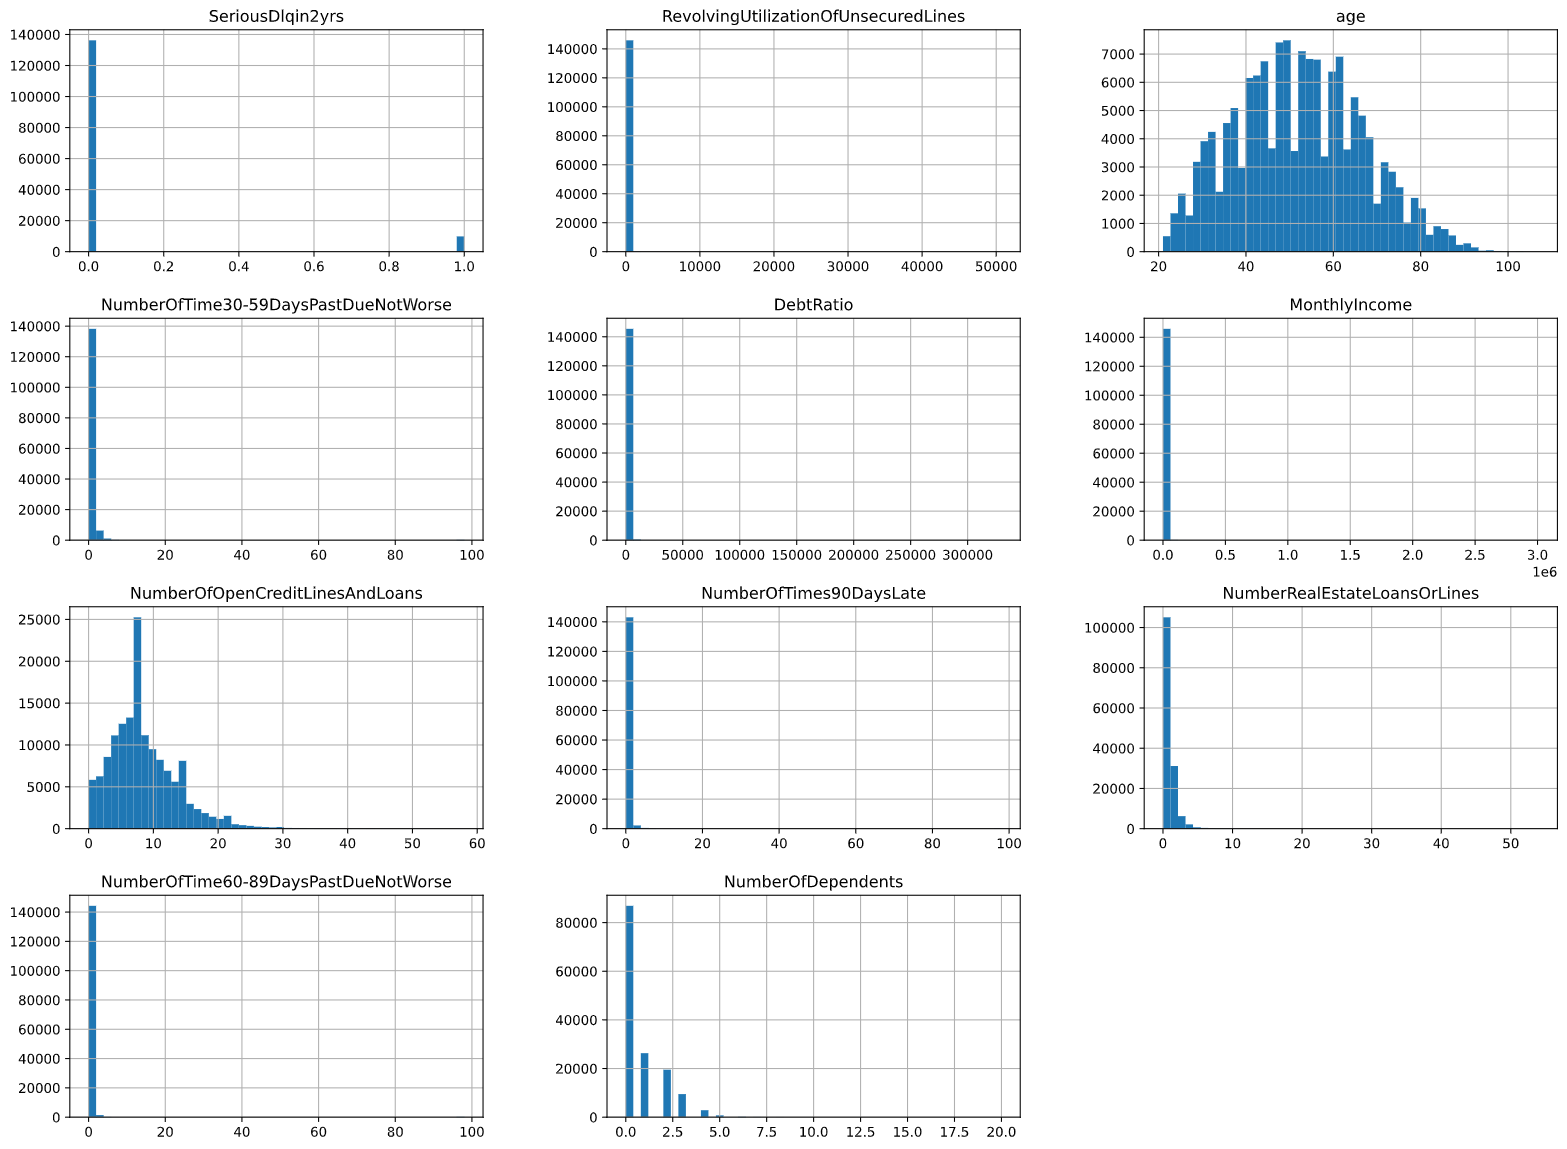
\includegraphics[width=0.6\textwidth]{zhifang.png} %1.png是图片文件的相对路径
	\caption{用于数据清洗的数据直方图} %caption是图片的标题
	\label{1} %此处的label相当于一个图片的专属标志,目的是方便上下文的引用
\end{figure}
\subsubsection{RevolvingUtilizationOfUnsecuredLines以及DebtRatio}
这两个属性单位为百分比,因此不应大于一,可将所有大于一的数据清除。
\subsubsection{Age}
该属性不能为0,且一般不大于150,因此我们只取(0,150)这一区间,其它的清除。
\subsubsection{NumberOfTime...}
NumberOfTime30-59DaysPastDueNotWorse, NumberOfTimes90DaysLate, \\NumberOfTime60-89DaysPastDueNotWorse这三项在直方图中不太清楚,
画为箱线图\ref*{2}后能够明显的看到它们的异常值均在80以上,因此我们只保留用户三项属性的值小于等于80的部分。
\begin{figure}[htbp]
	\centering
	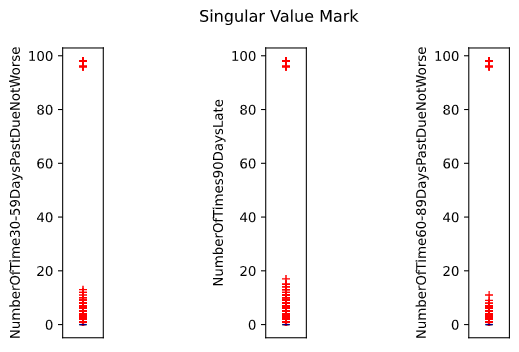
\includegraphics[width=0.6\textwidth]{number.png} %1.png是图片文件的相对路径
	\caption{NumberOfTime...箱线图} %caption是图片的标题
	\label{2} %此处的label相当于一个图片的专属标志,目的是方便上下文的引用
\end{figure}
\subsubsection{NumberRealEstateLoansOrLines,NumberOfDependents}
通过从大到小试探出异常值的下确界的方式( NumberRealEstateLoansOrLines:>50 ; NumberOfDependents:>15)将其清除
\subsubsection{MonthlyIncome}
剔除月薪大于50000以上的异常值。
\subsection{数据集分析}
\subsubsection{部分属性的分布特征}
下面\ref*{3}是经过数据清洗后的数据直方图

\begin{figure}[htbp]
	\centering
	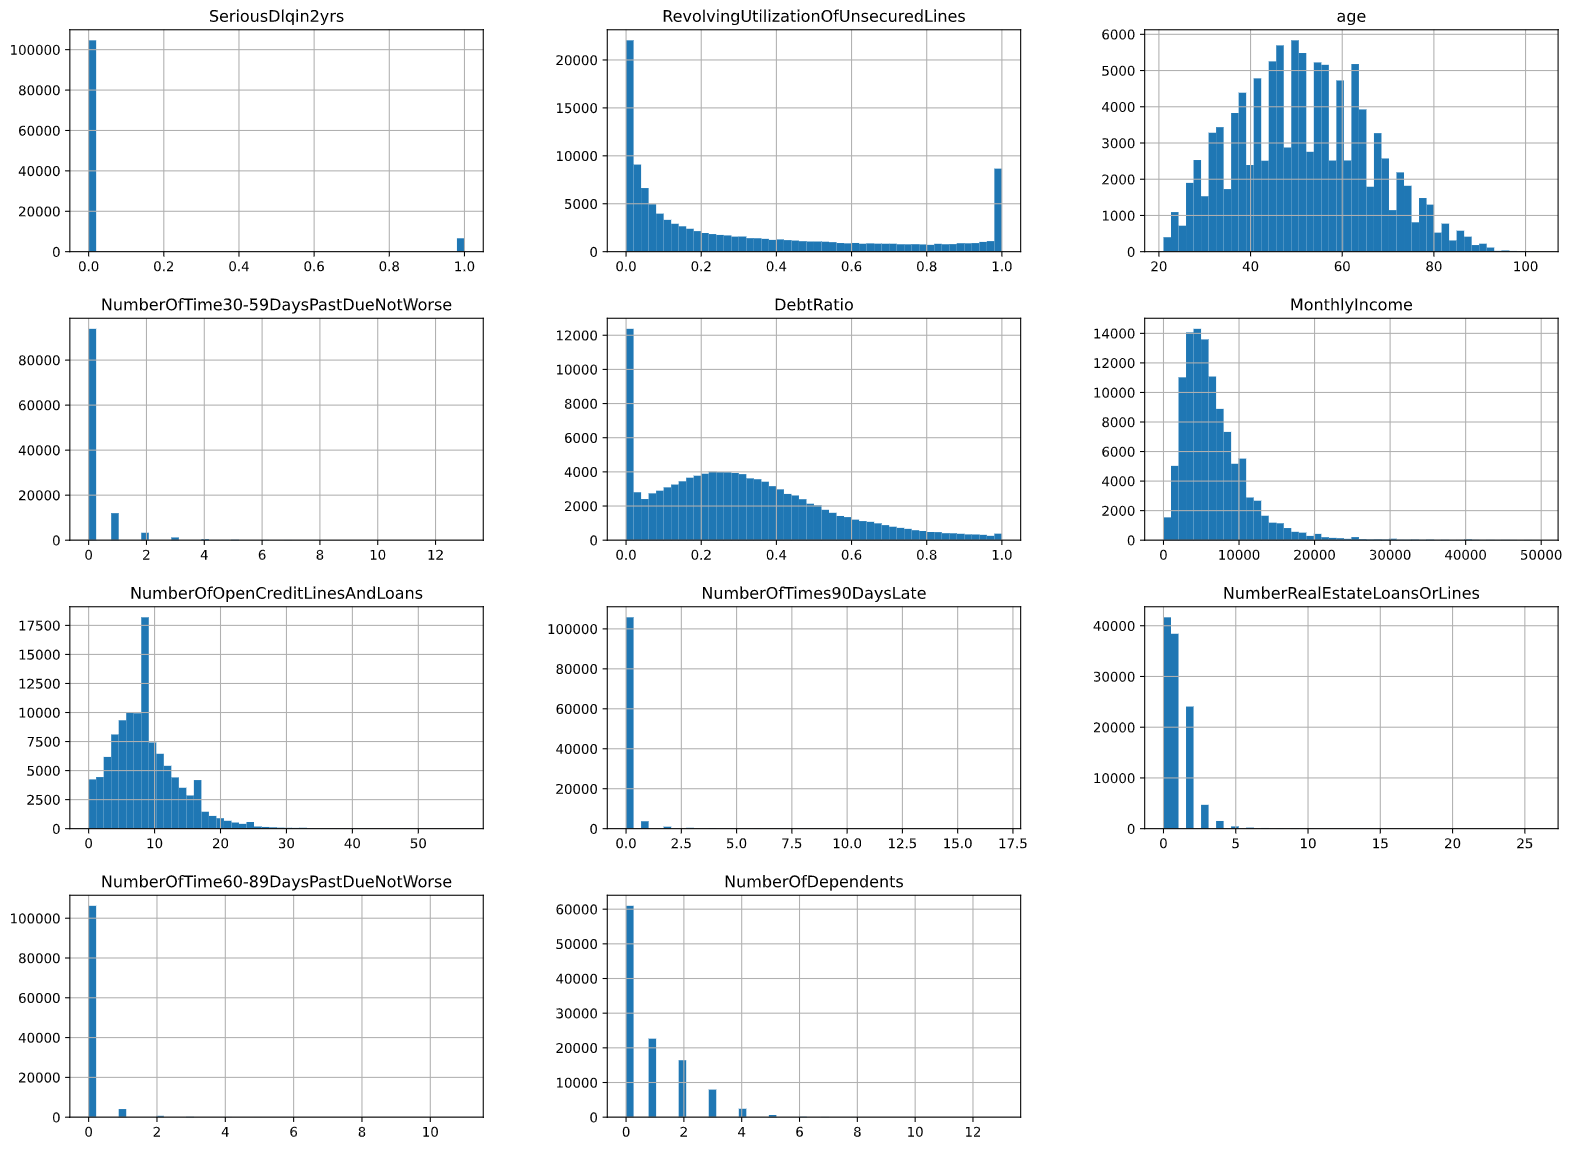
\includegraphics[width=0.6\textwidth]{zz.png} %1.png是图片文件的相对路径
	\caption{清洗后的数据直方图} %caption是图片的标题
	\label{3} %此处的label相当于一个图片的专属标志,目的是方便上下文的引用
\end{figure}

从\ref*{4}可以发现age, MonthlyIncome, DebtRatio, NumberOfOpenCreditLinesAndLoans 四个属性的的分布情况近似于正态分布,符合一般的统计假设。

\begin{figure}[htbp]
	\centering
	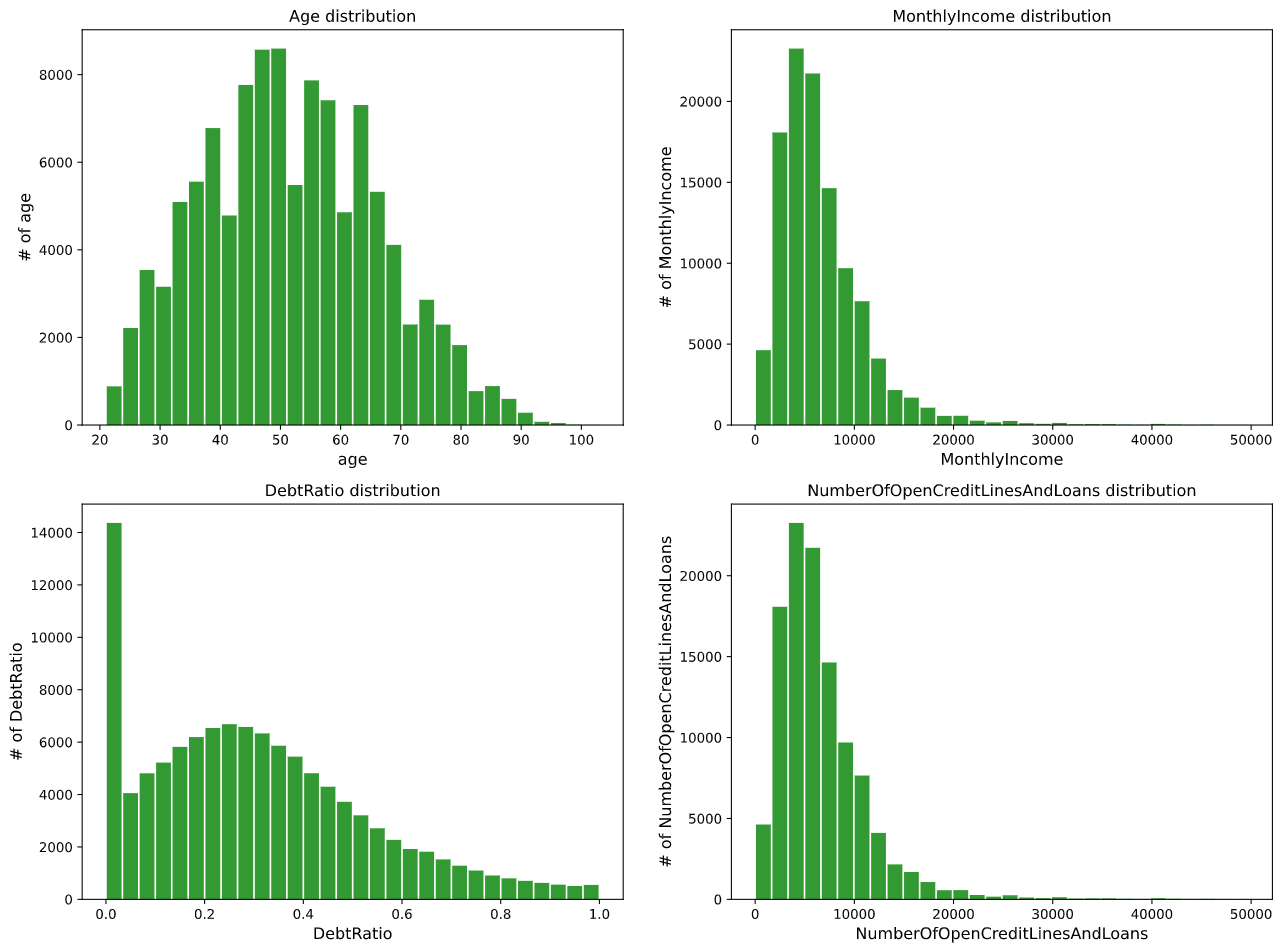
\includegraphics[width=0.6\textwidth]{dist.png} %1.png是图片文件的相对路径
	\caption{部分属性的分布特征} %caption是图片的标题
	\label{4} %此处的label相当于一个图片的专属标志,目的是方便上下文的引用
\end{figure}

如果只关注需要评估的SeriousDlqin2yrs的图像\ref*{5},会发现data中违约率的分布是相当不均衡,属于imbalanced classification问题

\begin{figure}[htbp]
	\centering
	
\includegraphics[width=0.6\textwidth]{ser.png} %1.png是图片文件的相对路径
	\caption{SeriousDlqin2yrs Plot} %caption是图片的标题
	\label{5} %此处的label相当于一个图片的专属标志,目的是方便上下文的引用
\end{figure}


\subsubsection{属性间的联系与特征}
通过计算属性间的相关性系数矩阵$R$,我们得到了它的相关性系数热力图\ref*{6}

\begin{figure}[htbp]
	\centering
	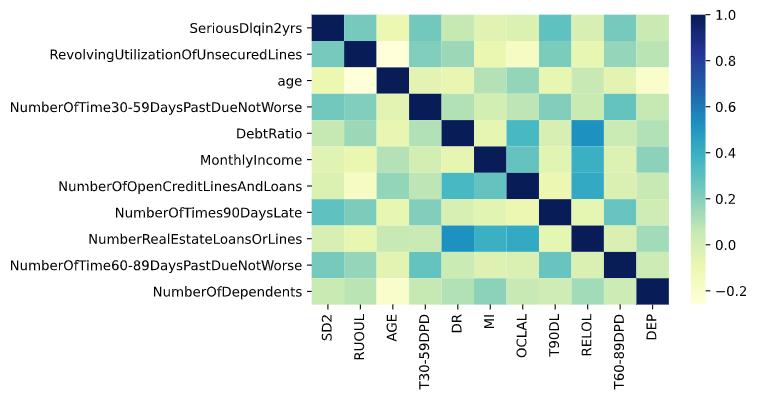
\includegraphics[width=0.6\textwidth]{cor.png} %1.png是图片文件的相对路径
	\caption{Correspondence Plot} %caption是图片的标题
	\label{6} %此处的label相当于一个图片的专属标志,目的是方便上下文的引用
\end{figure}

% Please add the following required packages to your document preamble:
% \usepackage{graphicx}
其相关系数矩阵为:


\begin{table}[htbp]
	\resizebox{\textwidth}{!}{%
		\begin{tabular}{|l|l|l|l|l|l|l|l|l|l|l|l|}
			\hline
			          & SD2    & RUOUL  & AGE    & T30-59DPD & DR    & MI    & OCLAL  & T90DL  & RELOL  & T60-89DPD & DEP    \\ \hline
			SD2       & 1.0    & 0.2375 & -0.096 & 0.2430    & 0.058 & -0.04 & -0.026 & 0.2961 & -0.013 & 0.2379    & 0.0440 \\ \hline
			RUOUL     & 0.2375 & 1.0    & -0.259 & 0.2093    & 0.149 & -0.08 & -0.166 & 0.2195 & -0.075 & 0.1654    & 0.0815 \\ \hline
			AGE       & -0.096 & -0.259 & 1.0    & -0.058    & -0.07 & 0.095 & 0.1715 & -0.075 & 0.0535 & -0.059    & -0.209 \\ \hline
			T30-59DPD & 0.2430 & 0.2093 & -0.058 & 1.0       & 0.102 & 0.006 & 0.0779 & 0.2031 & 0.0405 & 0.2812    & 0.0579 \\ \hline
			DR        & 0.0584 & 0.1490 & -0.079 & 0.1027    & 1.0   & -0.07 & 0.3540 & -0.012 & 0.5228 & 0.0374    & 0.1034 \\ \hline
			MI        & -0.046 & -0.085 & 0.0959 & 0.0069    & -0.07 & 1.0   & 0.2793 & -0.057 & 0.3962 & -0.029    & 0.1861 \\ \hline
			OCLAL     & -0.026 & -0.166 & 0.1715 & 0.0779    & 0.354 & 0.279 & 1.0    & -0.095 & 0.4248 & -0.022    & 0.0506 \\ \hline
			T90DL     & 0.2961 & 0.2195 & -0.075 & 0.2031    & -0.01 & -0.05 & -0.095 & 1.0    & -0.066 & 0.2716    & 0.0284 \\ \hline
			RELOL     & -0.013 & -0.075 & 0.0535 & 0.0405    & 0.522 & 0.396 & 0.4248 & -0.066 & 1.0    & -0.022    & 0.1384 \\ \hline
			T60-89DPD & 0.2379 & 0.1654 & -0.059 & 0.2812    & 0.037 & -0.02 & -0.022 & 0.2716 & -0.022 & 1.0       & 0.0332 \\ \hline
			DEP       & 0.0440 & 0.0815 & -0.209 & 0.0579    & 0.103 & 0.186 & 0.0506 & 0.0284 & 0.1384 & 0.0332    & 1.0    \\ \hline
		\end{tabular}%
	}
	
\end{table}


从系数矩阵中我们可以看出,和SeriousDlqin2yrs相关性较强的变量为RevolvingUtilizationOfUnsecuredLines、 NumberOfTime30-59DaysPastDueNotWorse、 NumberOfTimes90DaysLate、 NumberOfTime60-89DaysPastDueNotWorse

\subsection{具体实现}
\subsubsection{准备工作}
1、由于原始数据中违约率的分布是十分不均衡的,对于这样的不平衡分类问题,我们引入imlearn库,使用降采样RandomUnderSampler的手段使二者达到1:1平衡状态。

2、使用$train\_test\_split$函数对降采样后的数据集进行训练集与测试集的划分。

\subsubsection{训练拟合}
我们使用梯度下降树(GBDT)的方式进行训练拟合,并使用GridSearchCV进行参数上的优化调整。具体代码如下:
\begin{lstlisting}
param_search_1={'n_estimators':range(1,1002,100)}
sample=GridSearchCV(estimator=GradientBoostingClassifier(learning_rate=0.1,random_state=10),param_grid=param_search_1,scoring='roc_auc',n_jobs=-1,return_train_score=True,refit=True)
sample.fit(X_resampled,y_resampled)
sample.cv_results_,sample.best_params_,sample.best_score_
\end{lstlisting}
该段代码得到:
\begin{lstlisting}
	......(前略)
	{'n_estimators': 101},0.8401951053177882
\end{lstlisting}
前面的为GBDT中的参数在GridSearchCV中获得最大‘roc auc’值,也即后面的数字的参数。
该参数调整时范围较大,缩小范围继续调整
\begin{lstlisting}
param_search_1={'n_estimators':range(1,202,20)}
sample=GridSearchCV(estimator=GradientBoostingClassifier(learning_rate=0.1,random_state=10),param_grid=param_search_1,scoring='roc_auc',n_jobs=-1,return_train_score=True,refit=True)
sample.fit(X_resampled,y_resampled)
sample.cv_results_,sample.best_params_,sample.best_score_
\end{lstlisting}
得到
\begin{lstlisting}
	......(前略)
	{'n_estimators': 121},0.840527237620235
\end{lstlisting}

将该参数带入,继续调整其他参数,得到:
\begin{lstlisting}
	{'max_depth': 5, 'min_samples_split': 401},0.8405995893974124
	{'max_features': 5}, 0.8410558371623263
\end{lstlisting}
最后同步减小学习率提高决策树的数量:
\begin{lstlisting}
param_search_5={'n_estimators':[120,240,480,960,960*2],'learning_rate':[0.1,0.05,0.025,0.0125,0.00625]}
search_5=GridSearchCV(estimator=GradientBoostingClassifier(random_state=10,min_samples_split=401,max_depth=5,max_features=3), param_grid = param_search_5, scoring='roc_auc',n_jobs=-1)
search_5.fit(X_resampled,y_resampled)
search_5.cv_results_,search_5.best_params_,search_5.best_score_
\end{lstlisting}
在该参数上进行微调,得到最终的参数为:


$$
	min\_samples\_split=400
$$ 
$$
	max\_depth=4
$$ 
$$
	max\_features=8
$$ 
$$
	learning\_rate=0.025
$$ 
$$
	n\_estimators=480
$$

此时

$$
	train AUC Score: 0.8677278645422821
$$


\begin{figure}[htbp]
	\centering
	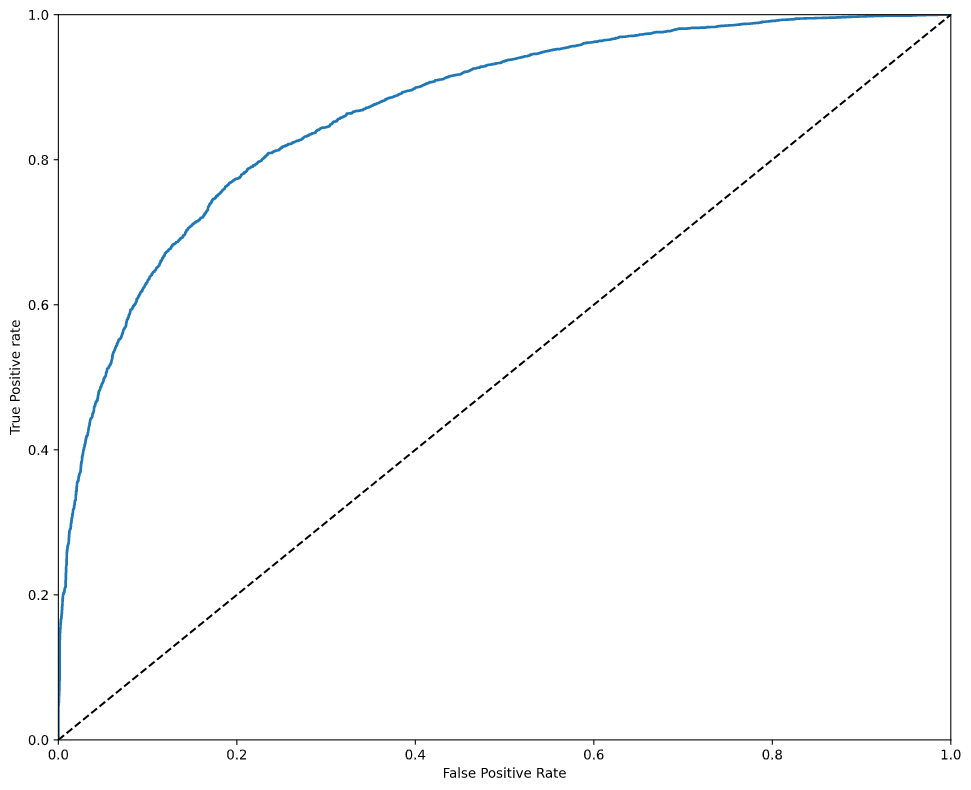
\includegraphics[width=0.6\textwidth]{train.png} %1.png是图片文件的相对路径
	\caption{TRAIN TPR-FPR曲线} %caption是图片的标题
	\label{7} %此处的label相当于一个图片的专属标志,目的是方便上下文的引用
\end{figure}

$$test AUC Score: 0.8354992323979017\\$$
\begin{figure}[htbp]
	\centering
	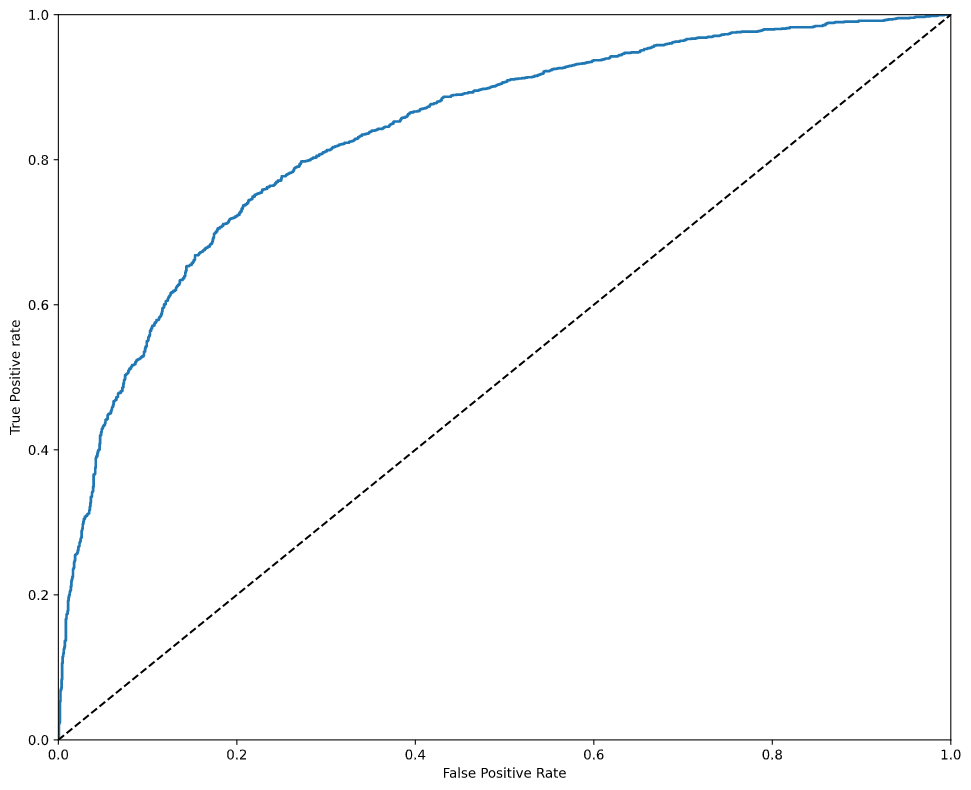
\includegraphics[width=0.6\textwidth]{test.png} %1.png是图片文件的相对路径
	\caption{TEST TPR-FPR曲线} %caption是图片的标题
	\label{8} %此处的label相当于一个图片的专属标志,目的是方便上下文的引用
\end{figure}

\subsection{可视化结果}
下面是我们做出的关于信用卡评分模型的可视化结果。

\begin{figure}[htbp]
	\centering
	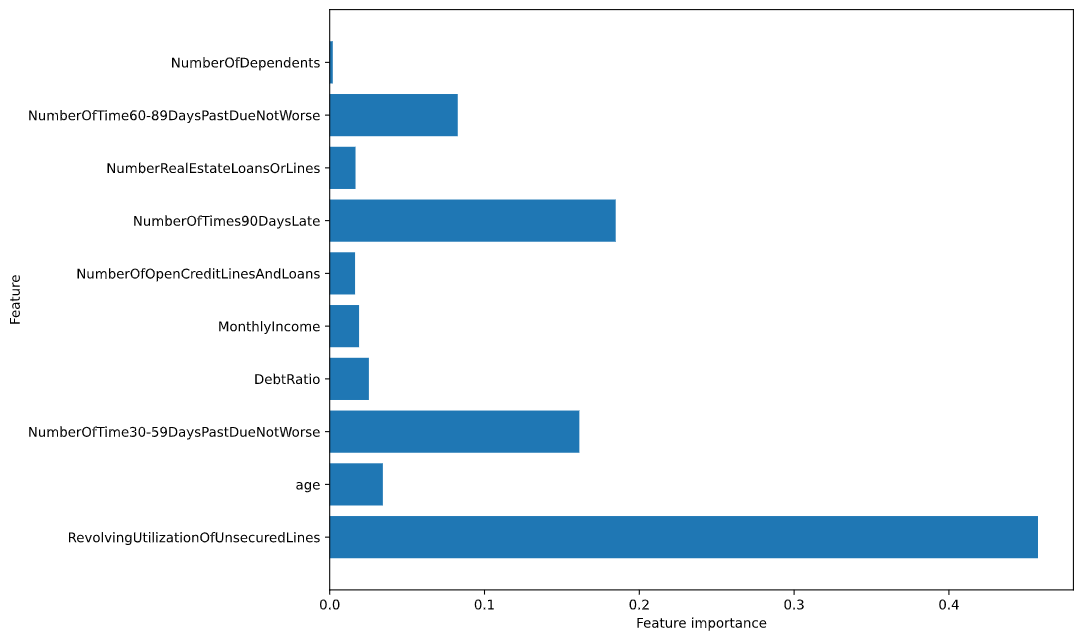
\includegraphics[width=0.6\textwidth]{imp.png} %1.png是图片文件的相对路径
	\caption{不同特征对用户信用评分的重要程度} %caption是图片的标题
	\label{9} %此处的label相当于一个图片的专属标志,目的是方便上下文的引用
\end{figure}

\begin{figure}[htbp]
	\centering
	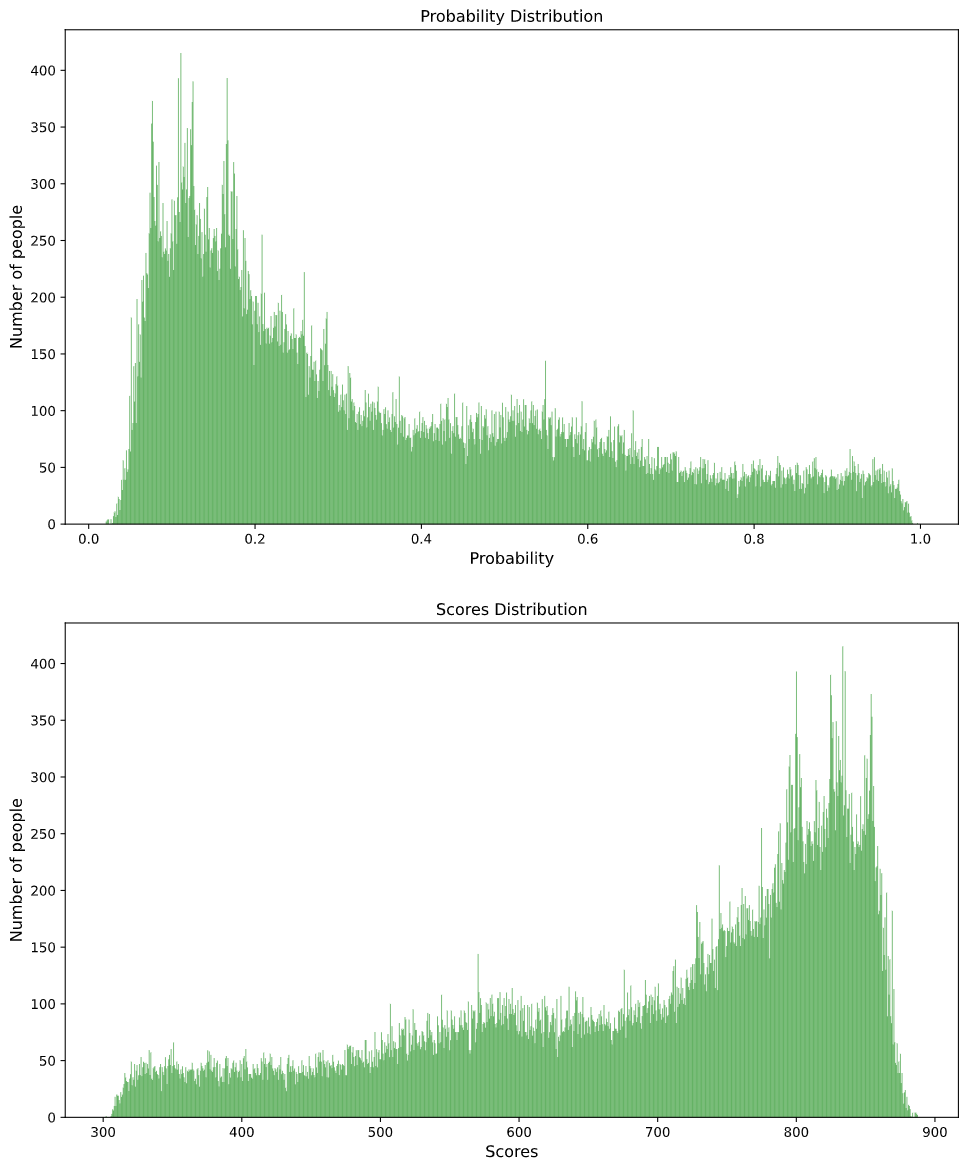
\includegraphics[width=0.4\textwidth]{pp.png} %1.png是图片文件的相对路径
	\caption{可能违约的概率密度以及对每个个体的评分} %caption是图片的标题
	\label{10} %此处的label相当于一个图片的专属标志,目的是方便上下文的引用
\end{figure}

\section{进行评估与预测}
导入'cs-test.csv',使用之前训练好参数的函数进行评估预测,并将函数返回的概率以线性的方式折合到个人评分上,形成最终的结论。

\section{结论}
通过上述的分析与计算,我们发现影响一个人是否违约的主要因素是其延期30-59天、60-89天、90天以上未偿付的次数,还有他的信用卡总余额和个人信用额度除以总信用限度的多少。反而个人的收入、背负债务的比重似乎在我们的分析下影响力显得并没有那么大。

\section{一些问题与讨论}
在进行数据处理的过程中,我们小组曾经想把对于MonthlyIncome缺省值的补全放在异常值剔除之后,因为这样做能够使随机森林算法在构建决策树时不会受到过多异常值的干扰,确实有道理。然而当我们动手实践之后,我们发现在中间过程完全一样的情况下,将补全缺省值放在最后做将会使训练集上的AUC下降2$\%$,测试集上的AUC下降近3$\%$。在进行了一番分析后我们发现,如果我们将异常值提前剔除,那么随机森林的OOB指标最小也
要大于-0.225,不然OOB只有-0.170。(二者均为$n\_estimators=600$时达到)因此也许正是由于拥有异常值的数据所贡献的“非异常值”对于模型的正向作用要大于其携带的异常值对于模型的负向作用要更强,导致了这种现象的发生。确实随机森林算法本质上是由许多个弱分类器“投票”组成的强分类器,因此可能对于奇异值、缺省值有较强的鲁棒性。

\section{分工}
\subsection*{罗文}
主要代码架构实现
\subsection*{刘华秋}
调参、对比不同方法,完善代码、报告写作、做PPT准备展示
\subsection*{顾逸鸥}
完善重要代码、进行项目规划、进度监督

% \begin{table}[]
% 	\begin{tabular}{|l|l|l|l|l|l|l|l|l|l|l|l|l|}
% 		\hline
% 		Training Data & ID           & SeriousDlqin2yrs    & RevolvingUtilizationOfUnsecuredLines & age                & NumberOfTime30-59DaysPastDueNotWorse & DebtRatio          & MonthlyIncome      & NumberOfOpenCreditLinesAndLoans & NumberOfTimes90DaysLate & NumberRealEstateLoansOrLines & NumberOfTime60-89DaysPastDueNotWorse & NumberOfDependents \\ \hline
% 		count         & 150000.0     & 150000.0            & 150000.0                             & 150000.0           & 150000.0                             & 150000.0           & 120269.0           & 150000.0                        & 150000.0                & 150000.0                     & 150000.0                             & 146076.0           \\ \hline
% 		mean          & 75000.5      & 0.06684             & 6.048438054666888                    & 52.295206666666665 & 0.4210333333333333                   & 353.00507576386985 & 6670.221237392844  & 8.45276                         & 0.26597333333333334     & 1.01824                      & 0.24038666666666667                  & 0.7572222678605657 \\ \hline
% 		std           & 43301.414526 & 0.24974553092871982 & 249.75537062544024                   & 14.771865863100349 & 4.192781272018315                    & 2037.81852314437   & 14384.674215282135 & 5.145950989643273               & 4.169303787594445       & 1.1297709848828605           & 4.1551794209872215                   & 1.1150860714871407 \\ \hline
% 		min           & 1.0          & 0.0                 & 0.0                                  & 0.0                & 0.0                                  & 0.0                & 0.0                & 0.0                             & 0.0                     & 0.0                          & 0.0                                  & 0.0                \\ \hline
% 		25\%          & 37500.75     & 0.0                 & 0.029867442                          & 41.0               & 0.0                                  & 0.17507383225      & 3400.0             & 5.0                             & 0.0                     & 0.0                          & 0.0                                  & 0.0                \\ \hline
% 		50\%          & 75000.5      & 0.0                 & 0.154180737                          & 52.0               & 0.0                                  & 0.366507841        & 5400.0             & 8.0                             & 0.0                     & 1.0                          & 0.0                                  & 0.0                \\ \hline
% 		75\%          & 112500.25    & 0.0                 & 0.5590462475                         & 63.0               & 0.0                                  & 0.86825377325      & 8249.0             & 11.0                            & 0.0                     & 2.0                          & 0.0                                  & 1.0                \\ \hline
% 		max           & 150000.0     & 1.0                 & 50708.0                              & 109.0              & 98.0                                 & 329664.0           & 3008750.0          & 58.0                            & 98.0                    & 54.0                         & 98.0                                 & 20.0               \\ \hline
% 	\end{tabular}
% \end{table}


% % Please add the following required packages to your document preamble:
% % \usepackage{graphicx}
% \begin{table}[]
% 	\resizebox{\textwidth}{!}{%
% 		\begin{tabular}{|l|l|l|l|l|l|l|l|l|l|l|l|l|}
% 			\hline
% 			Test Data & ID                & SeriousDlqin2yrs & RevolvingUtilizationOfUnsecuredLines & age                & NumberOfTime30-59DaysPastDueNotWorse & DebtRatio          & MonthlyIncome      & NumberOfOpenCreditLinesAndLoans & NumberOfTimes90DaysLate & NumberRealEstateLoansOrLines & NumberOfTime60-89DaysPastDueNotWorse & NumberOfDependents \\ \hline
% 			count     & 101503.0          & 0.0              & 101503.0                             & 101503.0           & 101503.0                             & 101503.0           & 81400.0            & 101503.0                        & 101503.0                & 101503.0                     & 101503.0                             & 98877.0            \\ \hline
% 			mean      & 50752.0           &                  & 5.310000296784993                    & 52.405436292523376 & 0.4537698393150941                   & 344.47502023825047 & 6855.0355896805895 & 8.453513689250563               & 0.29669073820478215     & 1.0130735052165947           & 0.27031713348373937                  & 0.7690463909705998 \\ \hline
% 			std       & 29301.53652398909 &                  & 196.15603864965954                   & 14.779756224905805 & 4.53848743193142                     & 1632.5952312454403 & 36508.60037459909  & 5.1441003376493875              & 4.5158586159249365      & 1.1102530938311783           & 4.5035776408513                      & 1.136778116728257  \\ \hline
% 			min       & 1.0               &                  & 0.0                                  & 21.0               & 0.0                                  & 0.0                & 0.0                & 0.0                             & 0.0                     & 0.0                          & 0.0                                  & 0.0                \\ \hline
% 			25\%      & 25376.5           &                  & 0.030130934499999998                 & 41.0               & 0.0                                  & 0.1734234825       & 3408.0             & 5.0                             & 0.0                     & 0.0                          & 0.0                                  & 0.0                \\ \hline
% 			50\%      & 50752.0           &                  & 0.152585671                          & 52.0               & 0.0                                  & 0.364259696        & 5400.0             & 8.0                             & 0.0                     & 1.0                          & 0.0                                  & 0.0                \\ \hline
% 			75\%      & 76127.5           &                  & 0.5642251414999999                   & 63.0               & 0.0                                  & 0.8516193055000001 & 8200.0             & 11.0                            & 0.0                     & 2.0                          & 0.0                                  & 1.0                \\ \hline
% 			max       & 101503.0          &                  & 21821.0                              & 104.0              & 98.0                                 & 268326.0           & 7727000.0          & 85.0                            & 98.0                    & 37.0                         & 98.0                                 & 43.0               \\ \hline
% 		\end{tabular}%
% 	}
% \end{table}
% \section{以下为一些工具}
% \begin{align}
% 	 & ABCDEFGHIJKLMNOPQRSTUVWXYZ \label{eq:alphabet}                                                                                                    \\
% 	 & abcdefghijklmnopqrstuvwxyz                                                                                                                        \\
% 	 & \alpha \beta \gamma \delta \epsilon \varepsilon \zeta \eta \theta \lambda \mu \nu \xi \pi \rho \sigma \tau \upsilon \phi \varphi \chi \psi \omega
% \end{align}
% \begin{align}
% 	\begin{bmatrix}
% 		1 & 2 \\
% 		3 & 4 \\
% 	\end{bmatrix}
% 	\begin{pmatrix}
% 		1 & 2 \\
% 		3 & 4 \\
% 	\end{pmatrix}
% 	\begin{matrix}
% 		1 & 2 \\
% 		3 & 4 \\
% 	\end{matrix}
% \end{align}

% \begin{equation}
% 	A_{t+1} = \arg\min_A \ \mathcal{L}(A,E_t,\Delta\tau_t,W_t,b_t), \nonumber
% \end{equation}

% \begin{equation}
% 	\begin{aligned} \label{eq:rasl}
% 		\min_{A,E,\Delta \tau} \quad & \sum_{i=1}^{N}||A_i||_* + \lambda ||E_i||_1                                                   \\
% 		\mathrm{s.t.} \quad          & D_i \circ \tau_i + \sum_{k=1}^{n_i} J_{ik} \Delta \tau_i \epsilon_k \epsilon_k^T = A_i + E_i, \\
% 		                             & i = 1,2,\cdots,N.
% 	\end{aligned}
% \end{equation}

% \begin{table}[htbptbp]
% 	\caption{Title of table} \label{tab:table}
% 	\centering
% 	\addtolength{\tabcolsep}{-0mm} % 控制列间距
% 	\begin{tabular}{ccccc}
% 		\toprule[0.75pt]	% package booktabs
% 		\multicolumn{4}{c}{table head}            \\
% 		\midrule[0.5pt]	% package booktabs
% 		\multirow{4}{*}{text} & 1  & 2  & 3  & 4  \\  % package multirow
% 		                      & 5  & 6  & 7  & 8  \\
% 		\cmidrule[0.5pt]{2-4}	% package booktabs
% 		                      & 9  & 10 & 11 & 12 \\
% 		                      & 13 & 14 & 15 & 16 \\
% 		\bottomrule[0.75pt]	% package booktabs
% 	\end{tabular}
% \end{table}
% 引用: Eq. \eqref{eq:alphabet}, Fig. \ref{figure:zju1},  \\


% \begin{algorithm}
% 	\caption{Title of the Algorithm}
% 	\label{algo:ref}
% 	\begin{algorithmic}[1]
% 		\REQUIRE some words.  % this command shows "Input"
% 		\ENSURE ~\\           % this command shows "Initialized"
% 		some text goes here ... \\
% 		\WHILE {\emph{not converged}}
% 		\STATE ... \\  % line number at left side
% 		\ENDWHILE
% 		\RETURN this is the lat part.  % this command shows "Output"
% 	\end{algorithmic}
% \end{algorithm}


\bibliographystyle{plain}
\bibliography{sample}
\end{document}